% \documentclass[twocolumn]{article}
\documentclass{article}

% Load basic packages
\usepackage{balance}  % to better equalize the last page
% \usepackage{graphics} % for EPS, load graphicx instead 
\usepackage{txfonts}
\usepackage{times}    % comment if you want LaTeX's default font
\usepackage{color}
\usepackage{textcomp}
\usepackage{booktabs}
%\usepackage{ccicons}
\usepackage{todonotes}
\usepackage{float}
\usepackage{url}  
\usepackage{titling}	% allows you to move title up the page
\usepackage[
  pdftex,
  colorlinks=true,
  pdfborder={0 0 0},
  linkcolor=red
]{hyperref}
\usepackage{xcolor} 
\usepackage{multicol}
\usepackage[margin=1in]{geometry}
\usepackage{graphicx}
\usepackage{capt-of}

% font  sizes
\usepackage{sectsty}			% set font sizes			
\sectionfont{\Large}			% (assumes default font size 10pt)
\subsectionfont{\large}
\subsubsectionfont{\large}
\paragraphfont{\normalsize}

% positioning
\setlength{\parindent}{0em}		% remove indent for new paragraph
\setlength{\parskip}{1em}		% space above paragraph
\setlength{\columnsep}{2em}		% distance between columns
\setlength{\droptitle}{-10em}

% llt: Define a global style for URLs, rather that the default one
\makeatletter
\def\url@leostyle{
  \@ifundefined{selectfont}{\def\UrlFont{\sf}}{\def\UrlFont{\small\bf\ttfamily}}}
\makeatother
\urlstyle{leo}

% This is a constant to space out the section titles from their body
\newcommand{\vspaceconst}{-2ex}

% For to do notes
\newcommand{\TODO}{\textbf{\textit{\textcolor{red}{TODO:}}} }

\title{Honours Project Report\\Fitness Logger with Micro-services}
\author{Dumitru Vulpe\\BSc (Hons) Applied Computing\\Supervised by Andrew Colby}
\date{May 2020}

\begin{document}

\maketitle


\vspace*{\fill/2}
\begin{abstract} 

This project is a tool to let people be able to log and track workouts overtime easily from their phone in a flexible yet complete way. The initial purpose was to make a phone application which can be used across different disciplines of sport and with different workout types. This would be done by breaking up the data in different manageable units so that the use can create their own workflow for logging workouts.

However, the main appeal of this project is the backend implementation. This is because as a part of the architecture design process, it was decided that a micro-services structure would be followed. Where the backend would be split up into multiple applications which would talk to each other where needed. This was chosen for a multitude of reasons, including as a learning experience for this kind of backend architecture.

\end{abstract}
\vspace*{\fill}

\newpage
\tableofcontents 
\newpage

\begin{multicols}{2}
\section{Introduction}
\vspace{\vspaceconst}

This project is split into two main objectives; first objective was to to be a learning experience of creating a full stack application beginning to end and more importantly to get into micro services backend development. The second objective was to attempt to solve a problem which exists in the fitness industry by creating an application which would be useful to a different range of people and potentially taking this product to the market.


\subsection{Why micro services}
\vspace{\vspaceconst}

The basic principle of micro services as supposed to a monolith, is to split up the backend application into multiple smaller application. For example, in theory, a service such as Amazon, could have a separate micro service for the cart function, one for listings, one more user account management, one for payment and more.
Micro services architectures are becoming more and more relevant simply because the industry is getting becoming more and more complex. And as size, complexity and user bases increase, so does the need for well scaled web applications. Micro services type architectures are simply one way to cleanly and easily scale web applications. So because of industry relevance and my personal enthusiasm, it was decided that this project's backend would also follow this architecture. 

\subsection{Creating a potential product}
\vspace{\vspaceconst}

Creating a folly fledged product out of this project was never my main idea. However, in my personal opinion, my planned solution for the problem has enough potential that could work as a product in the market. And as long as the application works as intended, there are multiple potential monetisation routes which could be taken, such as extra features behind a subscription or just a flat rate at purchase.

\subsubsection{The problem}
\vspace{\vspaceconst}

From personal past experience I have not found a simple, fuss free, yet flexible application for logging workout sessions and related notes for said session. The applications which I have tried so far are either made for a specific workout programs or are not complete, buggy or just do not have enough flexibility in the type of logging you can achieve. It often feels like a fight to be able to use such an app.\\
In the fitness world there can be a lot of different types of workouts, exercises, exercise variations, and ways to do said exercises. Because of this, coaches, personal trainers and everyday people usually would stick to using a notepad and paper  simply because there are no arbitrary restrains on what you can log.\\
Typically a notepad and pen is not a bad solution and usually preferable to most applications, however, there are certain drawbacks to this approach. One practical drawback is highlighted when working out in a commercial gym, walking around the gym using different equipment and carrying everything one might need including the notebook and pen combo can be quite cumbersome, same goes for actually noting down the data in the notebook. When it comes to looking back on previous workouts it can also be quite cumbersome, especially when you are in the middle of a workout and do not want to loose the tempo.\\

\subsubsection{My planned solution}
\vspace{\vspaceconst}

The idea was that the system would be designed around the data structure which would be saved by the user. This data structure would be made as simple as possible while still allowing all the common basic exercise options (such as repetitions, resistance values, sets etc) but also others (such as the option to just write a single value). Furthermore, the system would allow the user to create their own exercise types which they would then use when logging a workout. 

When using the application the user would first create a custom `type'. This type would usually be an exercise, however, it it not constrained to be one. For example, one type would be `exercise x' and another type could be `caffeine intake' for tracking the intake of caffeine over different workouts. Then, the 

\section{Background}
\vspace{\vspaceconst}

\subsection{Architecture design}
\TODO see if u can find a citation for the "popular questions to be answered" 

A lot of time during this project was allocated to research of the backend architecture design, specifically relating to micro services. And when it comes to it, there is not just one or few generally accepted standards and patterns that projects adopt. This is simply because each and every system architect needs to answer a lot of questions about it will all be built.
 For instance, the questions about how the different services should be split, some say it should be split by the feature, some say by the individual data element, by endpoint and more. Another popular questions is how the services diagram should look like, one of the popular answers are to have a separate authentication service to provide authentication for the application and proxy the requests to all the other services. However, regardless of the question, there are a lot of different ways solutions to all of these questions that need to be answered when starting a project using micro services and all of them come with their own advantages and disadvantages. 

\subsubsection{Helpful technologies}

When creating micro services systems, there are a lot of technologies which could and would be used to make the development of these services easier. Probably one of the first pieces of technologies to ease the development and deployment of micro services a lot easier was containers. Containers allow you to package applications with all of the needed dependencies and environments, they virtualise the user-land applications and share the hosts kernel, and on a Linux system that means that containers can virtually run anywhere. Furthermore, we have also have container management and orchestration solutions such as Docker\cite{Docker}, docker-compose\cite{Docker}, Kubernetes\cite{k8s} and more. These help with running the actual containers, and in the case of Kubernetes, it also allows us to easily define configurations and scale the containers either on a definition or on demand. Scaling here would be done by running more instances of that container across a cluster of machines running the Kubernetes and load balancing the traffic amongst them. This is known as horizontal scaling.\\
Micro services would often also need to talk to each other and as before, depending on requirements and design, there are different ways to do it. Overall there are two options many systems using both synchronous and asynchronous calls. Synchronous calls are usually straight forward and done over HTTP and the only thing that would need to be solved is proper authentication. Asynchronous calls are often made with either RPC calls (commonly gRPS\cite{grpc} would be used) or a message/event bus system such as Kafka\cite{kafka}. 

  Another great series of helpful technologies are service meshes, they provide great insight into your cluster of micro services. It is a dedicated infrastructure layer that all the different micro services would proxy their communication in-between. This can provide a multitude of benefits including communication observability, call chain traceability, secure connections and more. Examples of such services are Linkerd\cite{linkerd} and Istio\cite{istio}.

\subsection{Market} % Competitors apps

\TODO Need to find and list of competitor apps\\
- the one I have tried was zero to hero\\

\section{Specification}
\vspace{\vspaceconst}

\begin{verbatim}
This will be split into two problems
  - one being the scalability
    - warranting the micro services
  - the other being the flexibility part of the workout logging
    - explain how each user can create their own types which could be anything not just exercises with their own defined measurement units and more. 
    - could even talk about my initial idea of creating a highly flexible tagging system which can be searched
\end{verbatim}

The proposed project is tackling two main problems, one being a conceptual problem as a part of backend architecture which would need to be tackled in the future in case of heavy use or in case of the product getting multiple development teams. This problem is more of a conceptual proof of concept, that it could be done with relatively low complexity but yet giving us all of the benefits of micro services.

And the other problem being or concept and usability. The backend problem consists of scalability of the application.

\newpage

\section{Design}
\vspace{\vspaceconst}

\begingroup
\centering
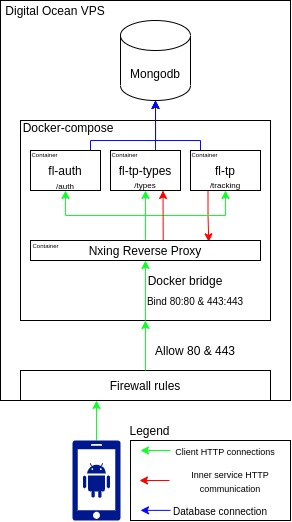
\includegraphics[width=0.7\linewidth]{./charts/fitness-logger.jpg}
\captionof{figure}{Fitness Logger Architecture}
~\label{fig:a}
\endgroup




% % NOTE: In order to tackle the main problem of simplicity and flexibility it was decided that the data would be atomised as much as possible, 

% \section{Implementation and Testing}
% \vspace{\vspaceconst}

% \section{Evaluation}
% \vspace{\vspaceconst}

% \subsection{Usability}
% \vspace{\vspaceconst}

% \subsection{Other Criteria}
% \vspace{\vspaceconst}

% \section{Description of the Final Product}
% \vspace{\vspaceconst}

% \section{Reflection}
% \vspace{\vspaceconst}

% \section{Conclusion}
% \vspace{\vspaceconst}

% \section*{Acknowledgements}
% \vspace{\vspaceconst}

\newpage
\begin{thebibliography}{9}

  \bibitem{Docker}
  Docker (Software) Wikipedia (2021).\\
  \url{https://en.wikipedia.org/wiki/Docker_(software)}

  \bibitem{k8s}
  Kubernetes website (2021).\\
  \url{https://kubernetes.io/}

  \bibitem{grpc}
  gRPC website (2021).\\
  \url{https://www.grpc.io/}

  \bibitem{kafka}
  Kafka website (2021).\\
  \url{https://kafka.apache.org/}

  \bibitem{linkerd}
  Linkerd website (2021).\\
  \url{https://linkerd.io/}

  \bibitem{istio}
  Istio website (2021).\\
  \url{https://istio.io/}
\end{thebibliography}

\section*{Appendices}
\vspace{\vspaceconst}

\end{multicols}
\end{document}
